% Author: Dominik Harmim <xharmi00@stud.fit.vutbr.cz>

\documentclass[10pt, hyperref={unicode}]{beamer}

\usepackage[czech]{babel}
\usepackage[utf8]{inputenc}
\usepackage{times} % font
\usepackage{listings} % algoritmy
\usepackage{xcolor} % definice vlastních barev
\usepackage{graphics} % vkládání obrázků
\usepackage{booktabs} % kvůli toprule, midrule a bottomrule

% téma prezentace
% metropolis progressbar bug - kvuli tomu je na každém snímku varování Overfull \hbox
\usetheme[progressbar=frametitle]{metropolis}
% číslování aktuální snímek/celkem snímků
\setbeamertemplate{footline}[frame number]

% definice vlastních barev
\definecolor{commentgray}{RGB}{150,152,150}
\definecolor{keywordpurple}{RGB}{167,29,93}
\definecolor{stringblue}{RGB}{24,54,145}
% nastavení listings
\lstset{
	basicstyle=\footnotesize,
	commentstyle=\color{commentgray},
	frame=single,
	keepspaces=true,
	keywordstyle=\color{keywordpurple},
	language=PHP,
	morekeywords={new, use},
	numbers=left,
	stringstyle=\color{stringblue},
	showstringspaces=false,
	showspaces=false,
	showtabs=false,
	tabsize=4,
}


\title{Typografie a~publikování\,--\,5.~projekt}
\subtitle{Nette Database}
\author{Dominik Harmim\texorpdfstring{\\ xharmi00@stud.fit.vutbr.cz}{}}
\date{\today}
\institute
{
	Vysoké učení technické v~Brně\\
	Fakulta informačních technologií
}


\begin{document}


\maketitle



\begin{frame}{Přehled}
	% číslovaný obsah
	\setbeamertemplate{section in toc}[sections numbered]
	% skrytí podsekcí v obsahu
	\tableofcontents[hideallsubsections]
\end{frame}




\section{Seznámení s~Nette Database}

\begin{frame}{Nette Database}
	\begin{itemize}
		\item
			Nette Framework, webový framework pro PHP, poskytuje vrstvu \alert{Nette Database} pro
			výrazně pohodlnější práci s~databázemi.

		\item
			Co umí?
			\begin{itemize}
				\item Snadno skládat databázové dotazy.
				\item Snadno získávat data.
				\item Pokládá efektivní dotazy a~nepřenáší zbytečná data.
			\end{itemize}
	\end{itemize}
\end{frame}



\begin{frame}{Instalace}
	\begin{itemize}
		\item
			\alert{Nette Database} může být použita samostatně nebo společně s~celým Nette Framework.

		\item
			Pro samostatné použití je potřeba stáhnout zdrojové kódy. Existují 2 způsoby:
			\begin{enumerate}
				\item použití nástroje \alert{composer} (preferovaný způsob) \\
					\texttt{composer require nette/database}
				\item stažení archivu ze stránek Nette \\
					\texttt{https://nette.org/cs/download}
			\end{enumerate}

		\item
			Pro následné použití v~PHP je nutné vložit stažené zdrojové kódy do našeho programu
			PHP direktivou \texttt{include} nebo \texttt{require}.
	\end{itemize}
\end{frame}




\section{Připojení k~databázi}

\begin{frame}[fragile]{Vytvoření připojení}
	\begin{alertblock}{\texttt{Nette{\textbackslash}Database{\textbackslash}Connection}}
		\begin{itemize}
			\item Třída tvořící obálku nad \texttt{PHP:PDO}.
			\item Reprezentuje připojení k~databázi.
			\item Poskytuje základní funkcionalitu pokládání dotazů.
		\end{itemize}
	\end{alertblock}

\begin{lstlisting}
use Nette\Database\Connection;
$dsn = "mysql:host=127.0.0.1;dbname=nazev_databaze";
$user = "uzivatel";
$password = "heslo";
$options = []; // konfigurace pro PDO a pro ovladac
$connection = new Connection($dsn, $user, $password, $options);
\end{lstlisting}
\end{frame}



\begin{frame}{Podporované databáze}
	\begin{table}
		\caption{Podporované databázové servery}
		\begin{tabular}{ll}
			\toprule
			Databázový server & DSN jméno\\
			\midrule
			MySQL & mysql\\
			PostgreSQL & pgsql\\
			Sqlite 3 & sqlite\\
			Sqlite 2 & sqlite2\\
			Oracle & oci\\
			MS SQL (PDO\_SQLSRV) & sqlsrv\\
			MS SQL (PDO\_DBLIB) & mssql\\
			ODBC & odbc\\
			\bottomrule
		\end{tabular}
	\end{table}
\end{frame}




\section{Skládání databázových dotazů}

\begin{frame}[fragile]{Diagram databáze}
	\begin{figure}[h]
		\centering
		\scalebox{0.4}{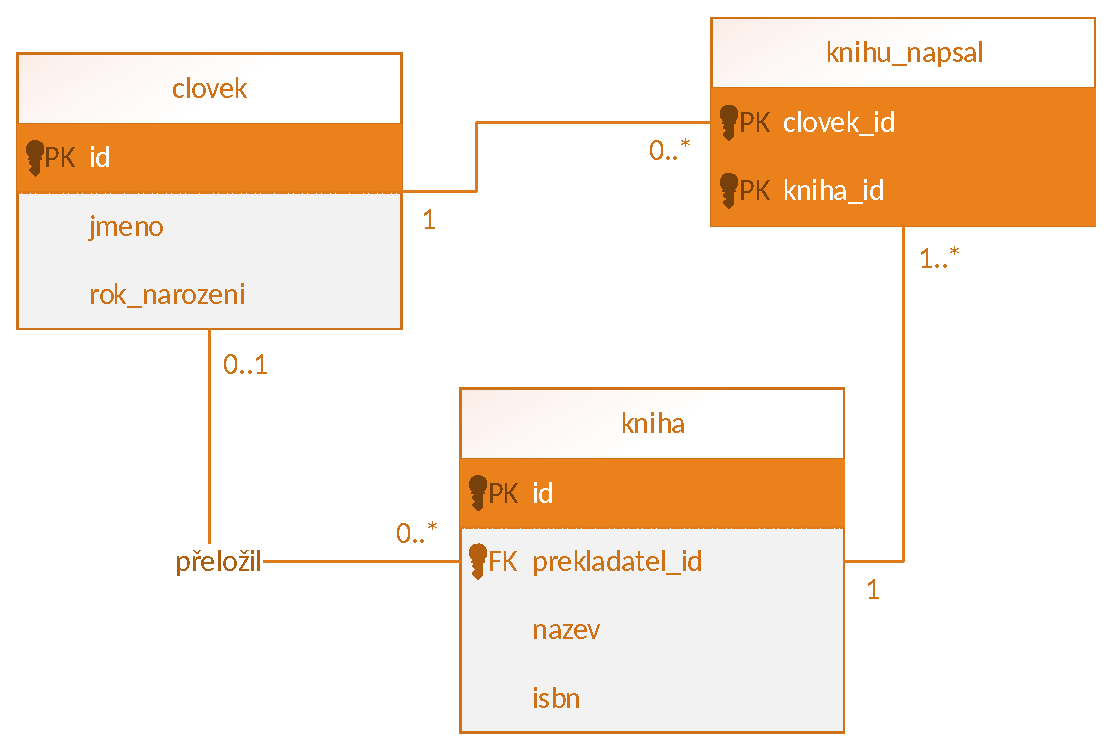
\includegraphics{img/db_diagram.eps}}
		\caption{Diagram databáze se kterou budeme pracovat v~následujících příkladech}
	\end{figure}
\end{frame}



\begin{frame}[fragile]{\texttt{Nette{\textbackslash}Database{\textbackslash}Connection query}}
	\begin{itemize}
		\item Jednoduché pokládání datábázových dotazů voláním metody \texttt{query}.
	\end{itemize}

\begin{lstlisting}[title=Změna názvu knihy s~ID 42:]
$data = ["nazev" => "Novy nazev"];
$connection->query("UPDATE kniha SET ? WHERE id=?", $data, 42);
\end{lstlisting}

\pause

\begin{lstlisting}[title=Výpis ISBN knihy s~ID 42:]
$result = $connection
			->query("SELECT * FROM kniha WHERE id=?", 42);
$book = $result->fetch();
echo "ISBN: " . $book["isbn"];
\end{lstlisting}
\end{frame}



\begin{frame}[fragile]{\texttt{Nette{\textbackslash}Database{\textbackslash}Table selection}}
	\begin{itemize}
		\item Jednodušší a~optimálnější způsob pokládání dotazů.
	\end{itemize}

\begin{lstlisting}[title={Výpis všech knih, jejich autorů a~překladatelů:}]
$books = $connection->table("kniha");
foreach ($books as $book) {
	echo "Kniha: " . $book->nazev;
	echo "Autori: "
	foreach ($book->related("knihu_napsal") as $wrote) {
		echo $wrote->clovek->jmeno;
	}
	if ($book->prekladatel) {
		echo "Prelozil: " . $book->prekladatel->jmeno;
	}
}
\end{lstlisting}
\end{frame}



\begin{frame}{Použité zdroje}
	\begin{thebibliography}{10}
		\bibitem[Nette Framework]{nette} Nette Framework
		\newblock \texttt{https://nette.org}

		\bibitem[Nette Framework, GitHub]{nette} GitHub: Nette Framework
		\newblock \texttt{https://github.com/nette/nette}

		\bibitem[Nette Database, GitHub]{nette} GitHub: Nette Database
		\newblock \texttt{https://github.com/nette/database}
	\end{thebibliography}
\end{frame}

\end{document}
